\chapter{INTRODUCTION} 
\label{chap1_intro}

This thesis explores the development of reinforcement learning based techniques specific to applications in nonlinear state estimation and Markov chain Monte Carlo (MCMC) algorithms. During the initial development of this thesis, nonlinear state estimation was the primary focus. Later, by lucky coincidence, it was observed that the same principles could be applied to obtain interesting results in MCMC algorithms as well. Hence, the chapter on MCMC forms a smaller portion of the thesis. In this chapter, the goal is a cursory introduction of the elements that are key to the problems considered in this thesis. We motivate the solution approaches adopted, without delving much into the technical details. 

\section{Nonlinear state estimation}
Consider a dynamic system evolving in time according to a given mathematical model. A complete characterization of the system is given by its \textit{states}. Uncertainties in the system model or external disturbances are modeled as process noise, and indirect observations of the state, corrupted by measurement noise are available. The observation model and the noise statistics are assumed to be known. The state dynamics and observations may be in either continuous or discrete time depending on the system properties. The state dynamics are assumed to be Markovian, i.e. in rough terms, the probability of the current state just depends on the previous state, and not on the entire history. 

A generic block diagram of a state estimator is depicted in \Fig{Fig:state_estimator}. The goal of any filtering/state estimation problem is to recursively estimate the states of the system based on noisy partial observations. The top row of the block diagram indicates the actual dynamics of the system. The \textit{prediction} and \textit{correction} blocks form part of the state estimator. Given the current estimate of the state, the prediction block gives the best state estimate, called the \textit{prior estimate} for the next time instant. The correction block updates it after receiving the most recent observation, and outputs the \textit{posterior estimate}. All filtering approaches share this basic structure, although in some cases, the prediction and correction steps may be combined.  

\begin{figure}
	\centering
	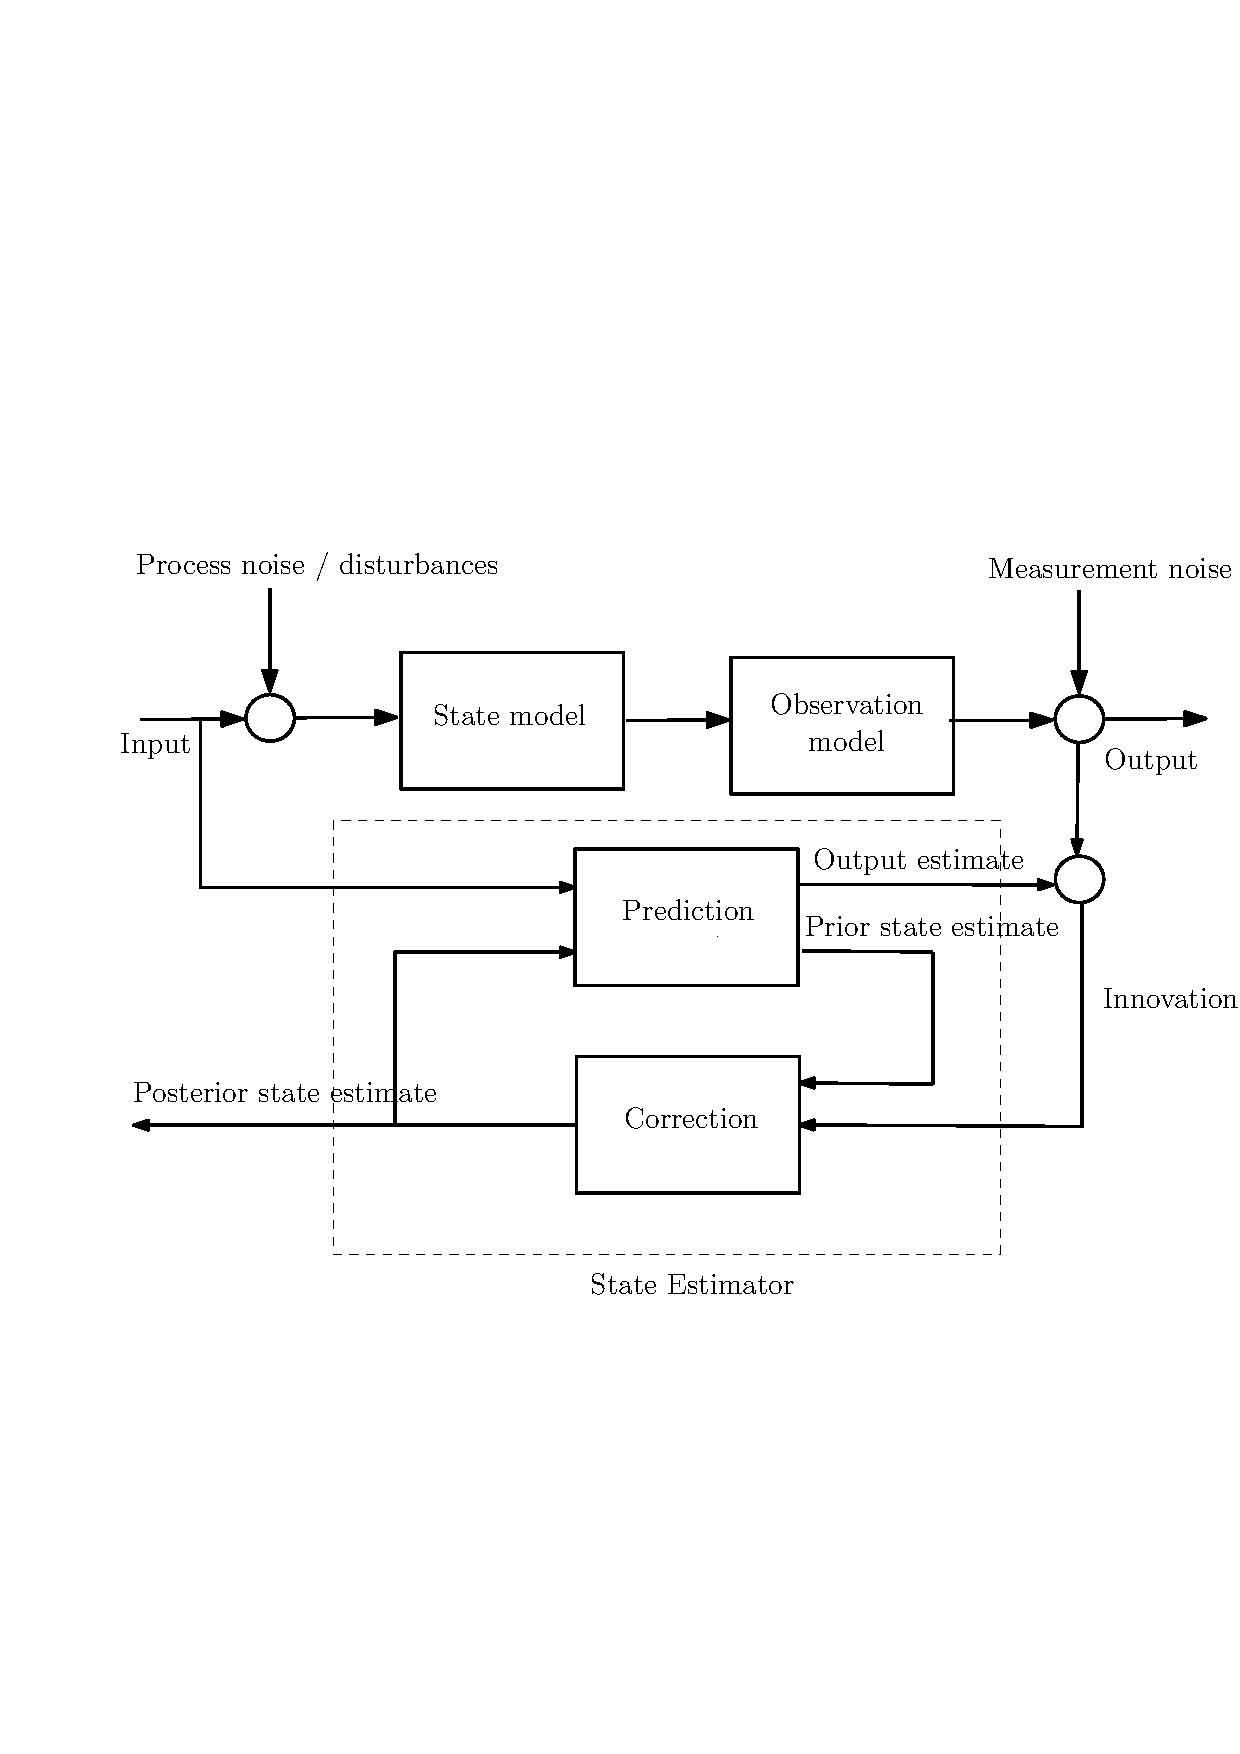
\includegraphics[width=7in]{images/Chap1_state_est_block}
	\caption{Block diagram of a state estimator}
	\label{Fig:state_estimator}
\end{figure}
Initial applications of filtering included satellite orbit determination, aircraft navigation and tracking \cite{kutsurpfi19}. More recently, filtering has found applications in diverse areas such as machine learning \cite{bishop06}, mathematical finance \cite{brihan08} and data assimilation problems for weather forecasting \cite{eve94}. 

When the system dynamics are linear and the noise quantities are Gaussian, the problem is simpler and the well-known Kalman filter is the optimal solution. The Kalman filter gives a linear SDE (stochastic differential equation) for the conditional mean of the state and a Riccati type ODE for the state covariance. However, in practice, the linear state dynamics - Gaussian disturbances assumption is often violated . For example, in weather forecasting the states evolve via a complex system of fluid mechanics equations that are nonlinear. The optimal solution is given by a set of SDEs, like the Zakai's equation or the Kushner-Stratonovich equation. A detailed discussion of the nonlinear filtering theory can be found in \cite{baicri08}. 

Linear approximations like the extended Kalman filter (EKF) were studied for application to nonlinear systems. They perform well as long as the state or observation dynamics do not deviate significantly from linearity. Later with the advent of modern computing, Monte Carlo based methods like the conventional bootstrap particle filter gained popularity. The underlying principle here is to approximate the posterior distribution using empirical samples called \textit{particles}. Budhiraja et al. \cite{budchelee07} provide a comprehensive survey of numerical methods for nonlinear filtering problems. 

The main focus of this thesis is a class of \textit{controlled particle system} algorithms called the feedback particle filter (FPF). Feedback particle filter was originally formulated for the continuous-time nonlinear filtering problem in the Euclidean setting \cite{yanmehmey13}. They have since been extended to Riemannian manifolds and matrix Lie groups \cite{zhatagmeh16}. The FPF is similar in its feedback structure to the Kalman filter and in its empirical approximation approach to the standard particle filter. In other respects, they are significantly different. A crucial component of the FPF is the \textit{gain function}, which is analogous to the Kalman gain in the Kalman filter. The optimal gain function in the FPF is obtained as the gradient of the solution to a particular version of \textit{Poisson's equation} \cite{yanmehmey13, laumehmeyrag14}. Obtaining an analytical solution to the Poisson's equation is often difficult and hence, approximation is required. In this thesis, our main focus is on developing algorithms to approximate the gain function. A detailed discussion is reserved for Chapter \ref{filtering}. 

\section{Markov chain Monte Carlo (MCMC) algorithms}
The second application of interest is Markov chain Monte Carlo (MCMC) algorithms. MCMC algorithms have a long history of being applied to problems in Bayesian statistics \cite{}. 

In standard Monte Carlo methods, expectation of a function $f$ of a random variable $X$ distributed according to a density $\pr$ is approximated empirically as,
\[
 \Expect_{X \sim \pr} [f(X)] := \int_\state f(x)\pr(x) dx \approx \frac{1}{N} \sum_{i=1}^N f(X_i) 
\]
where each $X_i$ is distributed according to $\pr$ and $N$ is sufficiently large. As is often the case, it may be difficult to generate a sequence of samples $\{X_i\}_1^N$ according to the desired \textit{target} distribution $\pr$. Methodologies such as \textit{rejection sampling} and \textit{importance sampling} make use of an easy-to-sample \textit{surrogate} distribution to sample from the original target distribution. But, if $\pr$ is high-dimensional, it is difficult to find a closely matching simple surrogate distribution. 

MCMC algorithms provide an alternative solution in this situation. They are a special class of Monte Carlo methods in which the samples $X_i$ are the states of an \textit{ergodic Markov chain}. Given the target density $\pr$, the problem reduces to finding an appropriate \textit{transition kernel} for a Markov chain that has $\pr$ as its \textit{invariant} density. The \textit{Langevin diffusion}, which is a perturbed gradient flow with respect to a potential function in continuous time, forms the basis of many such algorithms. The Gibbs algorithm \cite{tanwon87} and Metropolis-Hastings (M-H)  algorithm \cite{has70} are popular discrete-time examples belonging to this class. They have been widely applied for problems in Bayesian inference, statistical physics, computation biology etc.

%MCMC algorithms are a popular means of sampling from high dimensional densities. Typically, computing expectations of functions via integration is infeasible in high dimensions and MCMC algorithms provide a method to obtain numerical approximations to the expectation. 
The convergence of the empirical averages to the true expected value is guaranteed under general conditions by law of large numbers \cite{}. The main drawback of these techniques as compared to standard Monte Carlo sampling which provides independent and identically distributed (i.i.d.) samples, is that the successive samples of the Markov chain are correlated to each other. This results is slower convergence of the algorithms. The central limit theorem states that,
\[
\sqrt{N} \Bigl(\frac{1}{N} \sum_{i=1}^N f(X_i) - \Expect_{X \sim \pr} [f(X)] \Bigr) \overset{d}{\to} \normal(0, \asymvar^2),\qquad \text{as } N \to \infty, 
\]
where $\mathcal{N}(0,1)$ refers to the standard Gaussian distribution with mean zero and unit variance. \textit{Asymptotic variance} $\asymvar^2$ is a measure quantifying the rate of convergence. Lower its value, faster is the convergence of the Markov chain to its invariant distribution and hence, the goal is to minimize it. Asymptotic variance can be expressed in terms of the solution to Poisson's equation \cite{ctcn}. \textit{Control variates}, which are zero-mean terms added to the function $f$, have been used to reduce the asymptotic variance of the estimates without adding any bias. Henderson, in his thesis \cite{henthesis97} notes that the best choice of control variates can be constructed using the solution to Poisson's equation. They also feature prominently in Chapter 11 of the book \cite{ctcn} with the objective of constructing reduced-variance estimators for network models. Control variates constructed using the \textit{fluid value function} have been shown to produce a $100$-fold reduction in variance over the standard estimator for the KSRS queueing model. 

In this thesis, we demonstrate that the same algorithms we propose for approximating the FPF gain function, find additional application in improving the performance of popular MCMC algorithms. In \Section{poissons_eq}, we give a preliminary description of the Poisson's equation that is crucial to both our applications of interest.
% Section 11.2.1 and Section A.5 of CTCN, 
% Control variates - Prop 8.2.4 and Theorem A.5.4

\section{Poisson's equation} 
\label{poissons_eq}
In its most general form, Poisson's equation is a second-order differential equation of the form,
\begin{equation*}
\generate h := - f,
\end{equation*}
where $\generate$ is a second-order differential operator. Usually, $f$ is given and is ``centered'' by subtracting its mean. The function $h$ is unknown and solves the Poisson's equation. Poisson's equation appears widely in the context of Markov chains and stochastic optimal control. In the context of a diffusion processes, the operator $\generate$ refers to the \textit{infinitesimal generator}, also called the \textit{differential generator}. 

If $f$ is a one-step cost function, $h$ is called a \textit{relative value function} and is central to average-cost optimal control theory.  Relative value function gives the infinite-horizon expected cost when starting from a given state. Approximate solutions to the equation lead to direct performance bounds of the control algorithm \cite{ctcn}. Explicit bounds on the solution $h$ have been obtained under general conditions of the chain in \cite{}.

Our interest lies in a particular version of Poisson's equation associated to the \textit{Langevin diffusion} process. Langevin diffusion is discussed in greater detail in \Section{langevin_diffusion} and \Section{langevin_mcmc}. Gradient of the solution to this equation is the optimal choice of the gain function associated with the FPF \cite{yanmehmey13}. In MCMC algorithms, as noted by Henderson \cite{henthesis97} and later by Dellaportas et al. \cite{delkon12}, the optimal control variates can be constructed from this solution. Thus, Poisson's equation and its solution are central to the goals of this thesis. 

Obtaining a closed form solution is difficult outside of special cases and this motivates the study of approximation algorithms. Various approaches have been studied such as the \textit{Markov semigroup approximation} by Taghvaei et al. \cite{tagmeh16a}. Finding an approximate solution falls within the framework of reinforcement learning and in particular, temporal-difference (TD) learning. In this thesis, we develop variants of TD-learning algorithm to obtain approximate solutions to the Poisson's equation.

% basis for much of ergodic theory of Markov chains \cite{ctcn}


\section{Reinforcement learning and TD learning}
\label{rl_td}
In this section, a brief overview of reinforcement learning algorithms is provided. Reinforcement learning algorithms have gained popularity over the last decade having achieved major successes in a wide variety of applications. In a general setting, reinforcement learning problems involve learning what actions to take in a given situation, so as to maximize a numerical reward (or equivalently minimize a numerical cost) over a time-horizon. The learned set of actions, called a \textit{policy} is a mapping from the state space to the action space. In a stochastic setting, this mapping is expressed in terms of probability of taking a particular action in a given state. The learning is performed based on interactions with the environment without any prior knowledge of the model. A whole variety of algorithms including Q-learning and temporal-difference (TD) learning belong to this category. 

Sutton and Barto write in their monograph \cite{sutbar98}, ``If one had to identify one idea as central and novel to reinforcement learning, it would undoubtedly be \textit{temporal difference learning}''. TD learning has been discussed in the context of value function estimation for a fixed policy in \cite{ctcn}. The goal here is to obtain approximations to the true value function from within a parameterized family of functions. The learning problem is thus reduced to finding the best approximation based on a chosen criterion from within this class. An appropriate evaluation criterion is chosen based on the context. In optimal control, the goal is to optimize performance over the class of policies, whereas in MCMC, minimizing the asymptotic variance is the chosen criterion. Section 11.5.2 of \cite{ctcn} presents the \textit{least squares} TD (LSTD) learning algorithm for the discounted-cost problem. The parameter values are updated recursively in the algorithm and they have been shown to converge asymptotically to the optimal values. In Section 11.5.4, the results are generalized to the average-cost setting, which involves the Poisson's equation . In this thesis, we follow the ideas presented in Section 11.5.2 to develop a new class of algorithms called \textit{differential} TD learning that approximates the gradient of the solution to Poisson's equation directly. The discussion here is limited to the Poisson's equation associated to the Langevin diffusion; however a more general version of the algorithm with applications in optimal control is presented by Devraj et al \cite{devmey16arXiv}.
 
% nonlinear parameterization in Section 11.5.3 
% average-cost TD learning based on \cite{kontsi03a}
\section{Reproducing kernel Hilbert space (RKHS)}
 If any insight about the structure of the true value function is available, this can be exploited in choosing an appropriate function class. Traditionally, TD learning has been tested on spaces spanned by a carefully chosen finite set of basis functions. However, there are no standard approaches to choosing the basis. One of the novelties of this thesis is the use of reproducing kernel Hilbert space (RKHS) as an approximating function space for TD learning algorithms. This simplifies the choice of problem dependent basis functions by making use of the information about particle locations effectively. 
 
Reproducing kernel Hilbert spaces form an important class of function spaces in learning theory \cite{aro50, schsmo01}. They are complete Hilbert spaces uniquely characterized by a \textit{kernel} function. The use of RKHS for function approximation provides us with greater flexibility and potentially a richer function class. Although optimization in an RKHS is typically infinite dimensional, they are endowed with useful properties that help us reduce the problem to finding a finite set of parameters via the \textit{representer theorem} \cite{kimwah71, schhersmo01}. A brief background of the RKHS theory along with properties that make them useful in this thesis is provided in \Chapter{}. 
 

\section{Outline of the thesis}
The various topics discussed in this chapter may seem distinct and disconnected. This thesis attempts to tie them together as it progresses. To summarize, we restrict our attention to approximating solutions of a particular version of the Poisson's equation. Differential TD learning algorithms using a finitely parameterized family of functions and an RKHS are studied and presented. Approximations obtained using these algorithms are tested and have been shown to improve the performance of the FPF and MCMC algorithms. 

The main contributions of this thesis that form the remaining chapters can be summarized as - i) development of differential TD learning algorithm, similar to LSTD in \cite{ctcn} to approximate the gradient of the solution to Poisson's equation directly in \Chapter{chap2_diff_td}, ii) refinement of this algorithm with a simpler resolution \cite{radmey18a} in \Chapter{}, iii) improving the performance of the algorithm by the use of RKHS in Chapter \ref{}, iv) applications to nonlinear filtering in \Chapter{} and MCMC algorithms in \Chapter{}. Finally, conclusions and scope for future work are included in \Chapter{}.  

\section{Notation}
$\bfmX:= \{X_t: t\ge 0\}$ is a stochastic process, evolving on the state space  $\state$, which is taken to be $\Re^d$, unless specified. 
The symbol $\pr$   denotes a probability density on $\state$, and $L^2(\state,\pr)$ is the Hilbert space of square integrable functions with the usual inner product,
$\langle \phi,\psi\big\rangle_{L^2}:=\int\phi(x)\psi(x) \pr(x)\ud x$, where $\phi$ and $\psi$ are scalar valued functions in $L^2(\state, \pr)$;
written $L^2$ when there is no risk of ambiguity.  The associated norm is
denoted   $\|\phi\|^2_{L^2}:=\langle\phi,\phi\rangle_{L^2}$. The inner product is extended to vector valued functions $f,g: \state \to \Re^d$ by defining, $\langle f, g \rangle_{L^2} := \sum_{k=1}^d \langle f_k, g_k \rangle_{L^2}$. Another Hilbert space $\clH$ will appear in the application of reproducing kernel Hilbert space theory with its inner product denoted   $\langle \varble, \varble \rangle_{\clH}$,  and induced norm    $\| \varble \|_\clH$. $C^k$ is used to denote the space of $k$-times continuously differentiable functions $f\colon\state\to\Re$,
$\nabla f $ denotes the gradient of a function $f\in C^1$, and $\Delta f$ the Laplacian for $f\in C^2$.

%The remainder of the thesis is organized as below. In Chapter \cite{}, we discuss the problem set up, i.e. the Poisson's equation for Langevin diffusions and introduce \textit{differential TD learning} to obtain approximate solutions. A simpler resolution to the problem is proposed and an algorithm derived using this resolution is presented in Chapter \cite{}. In Chapter \cite{}, we discuss the application to nonlinear filtering in detail along with some numerical results. The second application to MCMC algorithms is presented with numerical examples in Chapter \cite{}. Finally, we present conclusions and scope for future work in Chapter \cite{}. 
 


 

%\begin{figure}[htbp]
%  \centering
%    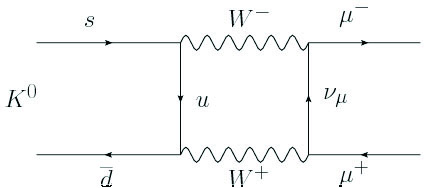
\includegraphics[width=5in]{images/diagram}
%    \caption[EPS format diagram. Note: no filetype is designated by adding an extension.]{EPS format diagram. Note: no filetype is designated by adding an extension. The file type is determined and the correct procedure is automatically chosen by xelatex.}
%\end{figure}
%
%
%
%\begin{figure}[htbp]
%     \centering
%   \mbox{
%      \subfigure [] {
\includegraphics[scale=0.6]{images/mouse}} \qquad
%      \subfigure []{
\includegraphics[scale=0.6]{images/mouse}} \qquad
%     }
%    \mbox{
%      \subfigure [] {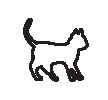
\includegraphics[scale=3]{images/cat}} \qquad
%      \subfigure [] {
\includegraphics[scale=0.6]{images/mouse}} \qquad
%      }
%    \caption[Tom and Jerry]{Tom and Jerries. This caption demonstrates how the sub-captions are left out of the List of Figures, but included in the figure itself. A) Tom the first; B) Tom the second; C) Jerry; D) Tom the third.}
%    \label{mice}
%  \end{figure}

